\section{Preliminary}
IMCL is an event-triggered language.
The purpose of IMCL modeling language design is to model the actual industrial control domain system.


\subsection{IMCL Mdodel}
The modeling of complex industrial systems has different angles.
The IMCL modeling method is based on the idea of refinement: modeling system functions, control logic, system resources, etc., layer by layer.

%下图表示的是使用 IMCL 简历一个复杂工控系统模型其系统结构,系统特性以元模型特点。

\begin{figure}[!htb]
  \centering
        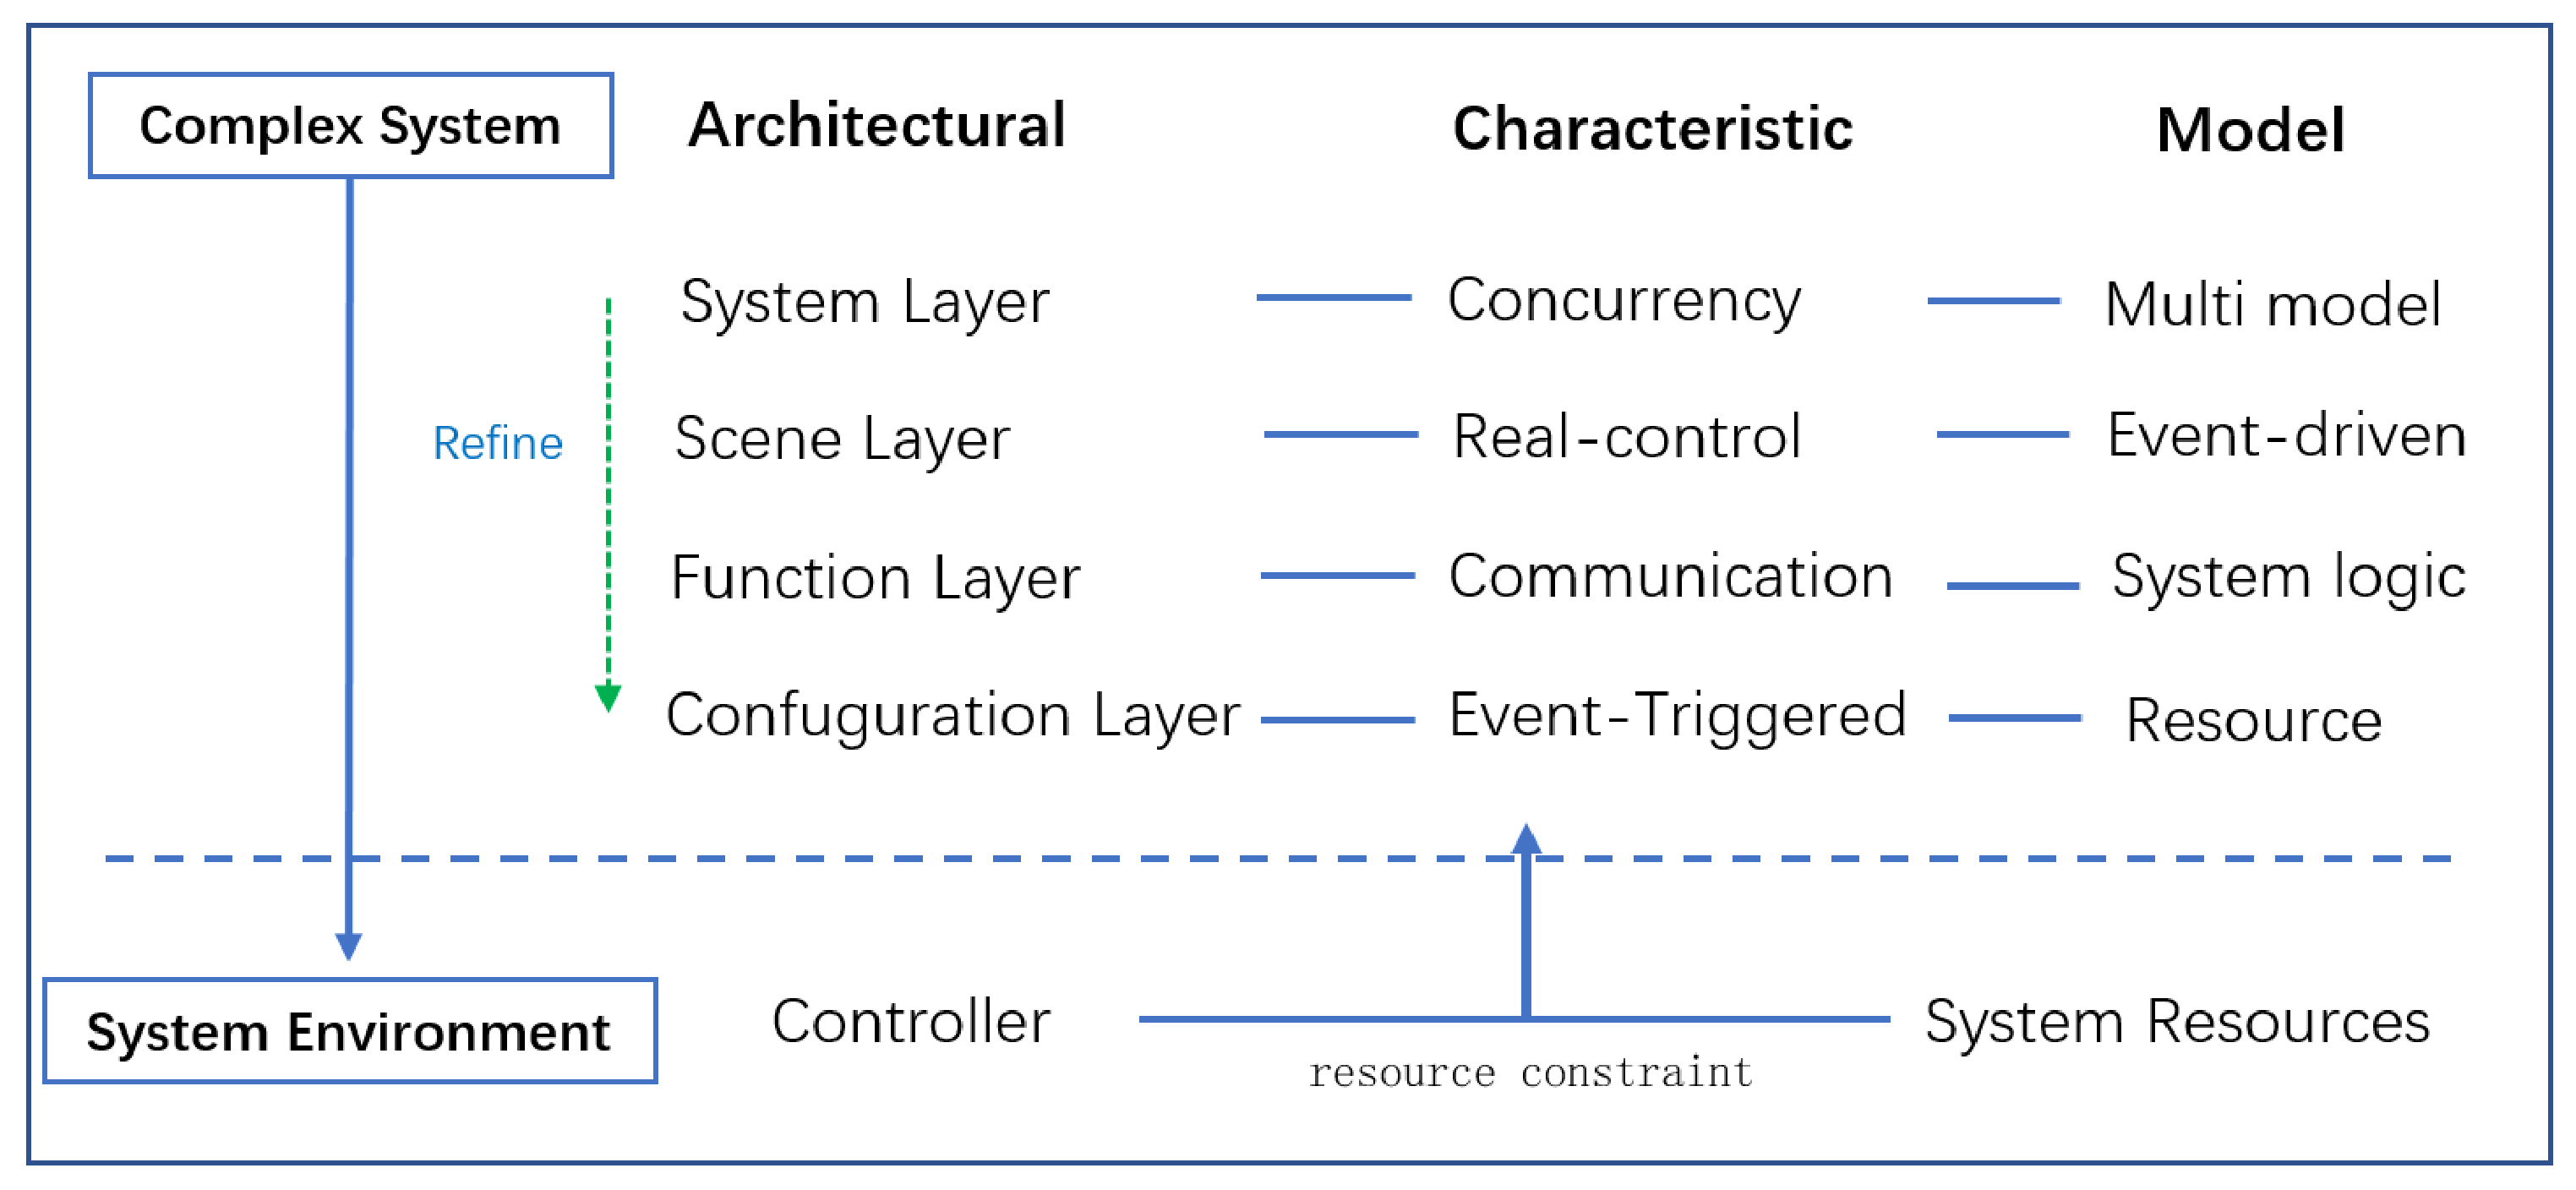
\includegraphics[height=1.4in, width=2.8in]{IMCLLayer}
  \caption{IMCL Model}\label{IMCLLayer}
\end{figure}


\begin{itemize}
  \item \textbf{System Layer} The system layer embodies the intuitive composition of a model. Usually, the system is composed of modular or functional components. For heterogeneous systems in the field of industrial control, controllers or processors with computational control capabilities within them can all run independently of each other. From the overall behavior of the system, the operation process is highly concurrent.
  \item \textbf{Scene Layer} The scenario layer describes the logical relationships between the independent components in the system, namely the control flow and interaction rules. All scenarios include system-specific task execution sequence, event triggering, message transmission, and so on. The running process of a system can be seen as the change of the scene, and can also be seen as the interaction process within the system. In the IMCL modeling process, the scene layer corresponds to events in the system.
  \item \textbf{Function Layer} The functional layer describes the system's behavioral process. Relative to the scene layer. The functional layer can be seen as the refinement of the scene layer. It describes the details of the implementation of the scene, including requests for various types of messages that occur in the scene, data calculations and interactions, and the scheduling relationships between the controller and the device.
  \item \textbf{Configuration Layer} The configuration layer reflects the mapping relationship between the computing unit with the control computing capability and the system physical resources in the system. Each computing unit can only control and schedule specific physical resources. The actual description of this constraint relationship is the respective functions of different processing units. By configuring this type of resource constraint relationship, the internal structure of a complex system can be more realistically reflected.
\end{itemize}

The entire system modeling process mainly includes the following three aspects:
\begin{enumerate}
  \item \textbf{Unified definition of resources} Representations of physical resources are different based on diverse industrial environment, for instance, sensors, read-write devices, and the other resources. Considering their effects on the whole system, we describe all those resources as variables to unifying definition of resources.
  \item \textbf{Modelling the system} Observing its behavior, the nature of the system is gathering functions, read-write operations, and other actions together. Similar to physical resources, we model them as execution expressions. Multiple execution expressions in one specific order can make up one trigger event
  \item \textbf{Resource Constraint}  It describes the constraints that physical resources are limited available for specific controllers.
\end{enumerate}

\subsection{IMCL formal model}
In order to better understand the characteristics of the IMCL model, we introduce the characteristics of the model from a formal point of view. For any system, modeling from the perspective of system trigger events using IMCL language, the system model can be expressed as follows:

\begin{displaymath}
Prog = \overset{n}{\underset{i=1}{\bowtie}} T_{i}, \ \ n \in N^{+}
\end{displaymath}

From the model refinement point of view, each system $Prog$ program can be seen as a set of trigger events, and then each trigger event $T_i$ is a set of ordered command expressions, each command expression can be seen as a system execution The smallest unit of calculation. For a system, the IMCL language is used for modeling from the perspective of system trigger events. The system model can be expressed as follows:

\begin{definition} \textbf{IMCL Model} $IMCL = \langle V, \ T^{*}, \ R^{*}, \ C^{*}\rangle$
\end{definition}
The IMCL model is characterized by event triggering and seen as a combination of events. The system variable $V$ is a set of different variables; $T^{*}$ is the event set, all events are distributed concurrently; $R^{*}$ represents the resource definition of the program, which is regarded as a special variable in the model; $C^{*}$ represents the resources constraint in the system relationship.

\begin{definition} \textbf{Variable} $V = V_{in} \cup V_{out} \cup V_{mess} \cup V_{local} \cup V_{res}$
\end{definition}
The set of variables represents how the variable data is expressed in the system. $V$ can be divided into five kinds of sets: the input variable set is represented as $V_{in}$, the output variable is $V_{out}$, the local signal variable is $V_{mess}$, the local variable set is $V_{local}$, and the physical resource description set $V_{res}$. These variables run through all state transitions during program execution and involve various types of operational rules for the system.

\begin{definition} \textbf{Trigger Event} $T = \langle id, \ c, \ E^{*}, \ V_t, \ R_t \rangle$
\end{definition}
$id$ represents the unique identifier of the event, each event can represent $T_{id}$;
$c$ is the event trigger condition and it can be a specific conditional expression or a bool value. It is a prerequisite for event execution migration.
$E^{∗}$ represents the set of tasks contained in the event;
$V_t = \{Vglobal; Vlocalg\}$ represents the set of variables contained in this event, where $V_{global}$ is the program global variable and $V_{local}$ is the set of local variables inside the event T.
$R_t \subseteq R^{*}$ indicates the physical resources that event mapped. The conditional triggering relationship of an event can be represented by the following expression:
    \begin{equation*}
        \normalsize
        \begin{aligned}
            (1)\langle id, c, E^{*}, V_t, R_t \rangle \rightarrow false \Rightarrow \langle id, c^{'}, E^{*},V_{t}^{'},R_t \rangle \\
            (2)\langle id, c, E^{*}, V_t, R_t \rangle \rightarrow true \Rightarrow \langle id, true, E^{*'},V_{t}^{'}, R_t \rangle
        \end{aligned}
    \end{equation*}


\begin{definition} \textbf{Task} $E = E_{com} | E_{inv} | E_{branch} | E_{loop} | E_{ch} | E_{sh}$
\end{definition}
The task represents the unit of program execution. Where $E_{com}$ represents a general assignment operation or numerical operation. $E_{inv}$ indicates that the task is to interact with system physical resources; $E_{branch}$ indicates conditional branch; $E_{loop}$ indicates program loop execution; $E_{ch}$ indicates execution statement of system communication process.


\begin{definition} \textbf{Branch} $E_{branch} = \langle b, \ E_{if}, \ E_{else} \rangle$
\end{definition}
The branch is the conditional statement, which means that the program enters the selected state. We define $b$ as the branch condition. $E_{if}$ will be chosen if b is true, otherwise the $E_{else}$. We define $e_0 \in E_{if}$ and $e_1 \in E_{else}$, $\vartriangle$  as the program execution current state, and $\vartriangle^{'}$ as the program change state. The program's transition relationship can be expressed in the following form:
\begin{equation*}
    \normalsize
    \begin{aligned}
        (1) \ &  \langle b, \vartriangle \rangle \rightarrow true, \langle e_0, \vartriangle \rangle \rightarrow \vartriangle^{'} \\
        & \Rightarrow \langle if \ b \ then \ e_0 \ else \ e_1, \vartriangle^{'} \rangle \rightarrow \langle e_0, \vartriangle^{'} \rangle\\
        (2) \ & \langle b, \vartriangle \rangle \rightarrow false, \langle e_1, \vartriangle \rangle \rightarrow \vartriangle^{'} \\
        & \Rightarrow \langle if \ b \ then \ e_0 \ else \ e_1, \vartriangle^{'} \rangle \rightarrow \langle e_1, \vartriangle^{'} \rangle
    \end{aligned}
\end{equation*}

\begin{definition} \textbf{Loop} $E_{loop} = \langle cond, E_{while} \rangle$
\end{definition}
Since the loop statement has been used to indicate that the current program enters a loop execution state, we define $b$ as a loop condition, $\vartriangle$ as the program execution current state, and $\vartriangle^{'}$ as the program change state. The execution of the program is as follows:
\begin{equation*}
    \normalsize
    \begin{aligned}
        (1)\ & \langle b, \vartriangle \rangle \rightarrow false \Rightarrow \langle while \ b \ do \ e, Δ\rangle \rightarrow \vartriangle \\
        (2)\ & \langle b, \vartriangle \rangle \rightarrow true, \langle c, \vartriangle \rangle \rightarrow \vartriangle^{''}, \langle while \ b \ do \ c, \vartriangle^{''} \rangle \rightarrow \vartriangle^{'} \\
        & \Rightarrow \langle while \ b \ do \ c, \vartriangle \rangle \rightarrow \vartriangle^{'}
    \end{aligned}
\end{equation*}


\begin{definition} \textbf{Communication} $E_{ch} = ch!V_{mess} |ch?V_{mess}$
\end{definition}
Where $ch!V_{mess}$ that send messages, is the active process of the program. $ch?Vmess$ that the system receives the message, is a similar to the ready-passive process. $\vartriangle$  is the current state of the program execution, $\vartriangle^{'}$ is the state of the program change. We represent the transmission mechanism of the communication.

$ch!Vmess$ defines the process as when the model is actively sending out messages, it will change the system message variables, modify the message variables, and the system state will change. The expression is as follows:
\begin{equation*}
    \normalsize
    \begin{aligned}
        \langle ch!, V_{mess}, \vartriangle \rangle \rightarrow \langle ch!, V_{mess}^{'}, \vartriangle^{'} \rangle
    \end{aligned}
\end{equation*}

$ch?V_{mess}?$ defines the process as the model is in the process of accepting the message, and its program state remains unchanged until it receives the target message from the channel.
\begin{equation*}
    \normalsize
    \begin{aligned}
        (1) \ & \langle ch!, b, V_{mess}, \vartriangle \rangle \rightarrow false \Rightarrow \langle ch!, b, V_{mess}^{'}, \vartriangle \rangle \rightarrow \vartriangle \\
        (2) \ & \langle ch?, b, V_{mess}, \vartriangle \rangle \rightarrow true, \langle c, \vartriangle \rangle \rightarrow \vartriangle^{''}, \langle ch?, b, V_{mess}, \vartriangle^{''} \rangle \\
         & \rightarrow \vartriangle^{'} \Rightarrow \langle ch?, b, V_{mess}, \vartriangle\rangle \rightarrow \vartriangle^{'}
    \end{aligned}
\end{equation*}

\begin{definition} \textbf{Schedule} $E_{sh} = \langle a_{data}, \lambda, Dev \rangle$
\end{definition}

The resource scheduling $E_sh$ reflects the scheduling relationship between the controller and the physical resources. There are two types of $\lambda$, $a_{data} \ll Dev$ and $a_{data} \gg Dev$. $a_{data} \ll Dev$ indicates that the controller schedules acquisition of data to the physical device; $a_{data} \gg Dev$ indicates that the controller schedules transmission of data to the physical device. Since the purpose of the IMCL model is to study the logical function of the system, we use the two forms of ε to describe the scheduling function between the controller and the physical device.

\subsection{Group model generation}

The specific implementation details of the population model generation technique have been proposed in our previous published papers. The advantage of using the ICML modeling method is that we can intelligently split a complex model into multiple sub-models given the constraints of the resource and controller constraints. The sub-models can communicate with each other and achieve the same function as the original model. The generated sub-models correspond to specific target platforms respectively, and the main research work in this paper is to realize the code generation work from the IMCL model to different target platforms.

